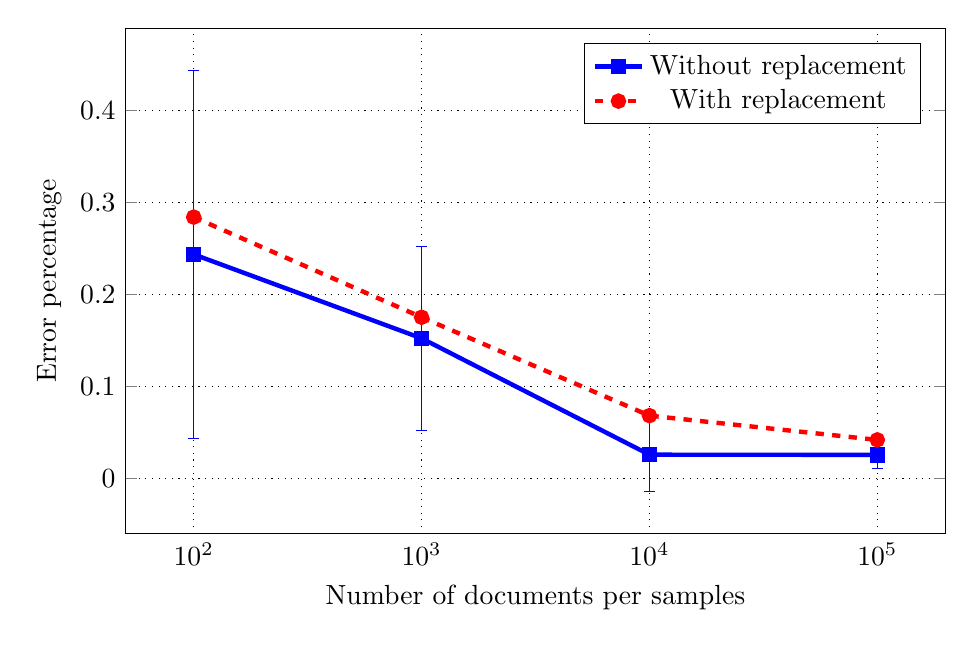
\begin{tikzpicture}
\begin{axis}[legend style={at={(0,0)},anchor=west,at={(axis description cs:1.05,0.45)}, every axis plot/.append style={ultra thick}},title={},
mark options={solid,scale=1},
xlabel={Number of documents per samples},
xmode = log,        % logarithmic x axis
ylabel={Error percentage},
%axis background/.style={fill,bottom color=gray!50,top color=white},
xtick style={draw=none},
grid=none,
height=8cm,width=12cm,
grid style={dotted,black},
legend pos=north east,
grid=major
]
\addplot[mark=square*,blue, error bars/.cd, y dir=both, y explicit] plot coordinates{
(100,0.243875) +=(0,0.2) -= (0,0.2)
(1000,0.152625) +=(0,0.1) -= (0,0.1)
(10000,0.0261373737) +=(0,0.04) -= (0,0.04)
(100000,0.026) +=(0,0.015) -= (0,0.015)
};
\addlegendentry{Without replacement}
\addplot[dashed,mark=*,red, error bars/.cd, y dir=both, y explicit] plot coordinates{ 
(100,0.284375)
(1000,0.175508425)
(10000,0.0686)
(100000,0.0422475)
};
\addlegendentry{With replacement}
\end{axis}
\end{tikzpicture}